%FOR PDFLATEX USE ONLY
\documentclass[a4paper,12pt]{article}

\usepackage{amssymb,amsmath} %math symbols

\usepackage[margin=2cm]{geometry} %paper geometry

\usepackage[T1, T2A]{fontenc}

\usepackage[utf8]{inputenc} %allows unicode (including russian) source file
\usepackage[russian]{babel} %docment in russian-style
\usepackage[utf8]{inputenc}
%\usepackage[unicode]{hyperref} %links inside of the text
\usepackage[pdftex]{graphicx} %includegraphics pictures
\usepackage{cmlgc} %bold text

\usepackage{array} %arrays

%\usepackage{wrapfig}
%\usepackage{array}
%\usepackage{lipsum}
%\usepackage{esvect}
%\usepackage{hyperref}

\usepackage{amsmath}
\usepackage{amssymb}
\usepackage{mathtools}
\usepackage{mathtext}

\usepackage{subfig}
%\usepackage{calc}
%\usepackage{pgfplots,tikz,circuitikz}
%\usepackage{tkz-euclide}

\begin{document}

\begin{center}
  \LARGE{Работа 3.4.4}\\[0.2cm]
  \LARGE{Петля гистерезиса (статический метод)}\\[0.2cm]
  \large{Малиновский Владимир}\\[0.2cm]
  \normalsize{\texttt{galqiwi@galqiwi.ru}}
\end{center}

\textbf{Цель работы:} Исследование кривых намагничивания ферромагнетиков с помощью баллистического гальванометра.\\
\textbf{В работе используются:} генератор тока с блоком питания, тороид, соленоид, баллистический гальванометр с осветителем и шкалой, амперметры, магазин сопротивлений, лабораторный автотрансформатор (ЛАТР), разделительный трансформатор.\\
\begin{center}
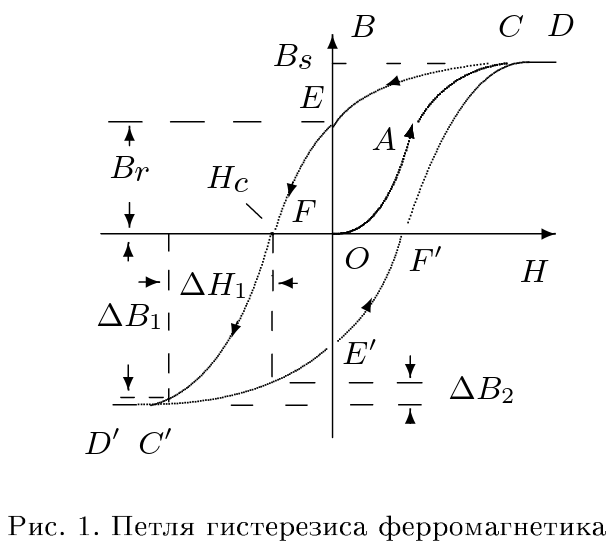
\includegraphics[width=0.60\textwidth]{1.png}
\end{center}
\section*{Идея}
Как показано на рисунке 1, зависимость напряженности $H$ и индукции $B$ в ферромагнетиках неоднозначная. В этой работе предстоит промерить этот эффект, используя гальванометр, работающий в баллистическом режиме.
\begin{center}
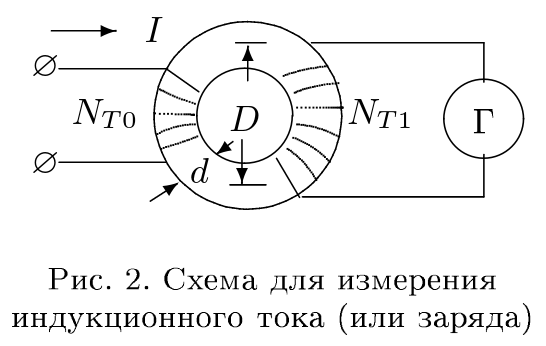
\includegraphics[width=0.60\textwidth]{2.png}
\end{center}
\newpage
На тороидальный сердечник (рис. 2) равномерно намотана намагничивающая обмотка с числом витков $N_{T0}$, а поверх нее -- измерительная обмотка с числом витков $N_{T1}$. Идея заключается в том, что, если быстро изменить ток в намагничивающей обмотке, то в измерительной обмотке возникнет ЭДС индукции. Причем, напряженность поля $H$ буждет пропорциональна току $I$ в первичной обмотке, а изменение магнитной индукции $B$ -- заряду, протекающему через гальванометр. Этот заряд пропорционален первому отбросу зайчика у гальванометра.
Для получения $H$ достаточно знать известные параметры установки:
$$H=\frac{N_{T0}}{\pi D}I,$$
где $D$ -- средний диаметр тора.\\
А вот для нахождения $B$ придется калибровать гальванометр:
\begin{center}
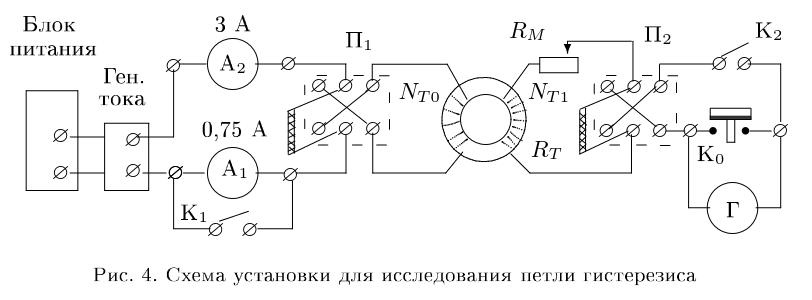
\includegraphics[width=0.80\textwidth]{3.png}
\end{center}
\begin{center}
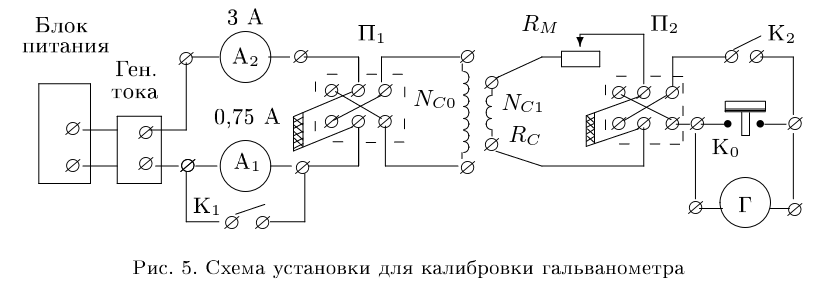
\includegraphics[width=0.80\textwidth]{4.png}
\end{center}
Верно, что
$$\Delta B = \mu_0 \left(\frac{d_c}{d_T}\right)^2\frac{N_{C0}}{N_{T1}}\frac{N_{C1}}{l_C}\Delta I_1 \frac{\Delta x}{\Delta x_1},$$
где $R_1$ и $R$ -- полные сопротивления соленоида и тороида соответственно, $l_C$ -- длина соленоида в калибровочной схеме, $d_c$ и $d_T$ -- диаметры соленоида и тороида соответственно, $\Delta x$ и $\Delta x_1$ -- баллистические показатели гальванометра при измерениях и калибровке соответственно, а $\Delta I_1=I_{max}$ -- ток, подаваемый при калибровке.
\section*{Метод и результаты}
Нумерация соответствует нумерации в лабнике.
\subsection*{1-2}
Соберем установку с рис.4 и измерим максимальный ток через амперметр $I_{max}=1462\pm3 \text{мА}$.
\subsection*{3}
Установим сопротивление $R_\text{М} = 90\,\text{Ом}$, так, чтобы при $R_\text{С} = 60\,\text{Ом}$, $R_\text{М}>R_\text{С}$. Выставим нулевое положение зайчика.
\subsection*{4-5}
Пройдемся по всей петле (от $I_{max}$ до $-I_{max}$ и обратно) и замерим значения тока $I$ и отклонение зайчика $\Delta x$:

\begin{center}
\begin{tabular}{|c|c|c|c|c|c|}\hline
$I\text{, mA}$&$\Delta I\text{, mA}$&$\Delta x\text{, у.ед}$&$I\text{, mA}$&$\Delta I\text{, mA}$&$\Delta x\text{, у.ед}$\\\hline
$1462$&$3$&$0$&$-1460$&$3$&$0$\\\hline
$515$&$1$&$-130$&$-515$&$1$&$137$\\\hline
$250.2$&$0.5$&$-112$&$-249.9$&$0.5$&$111$\\\hline
$157.0$&$0.3$&$-69$&$-156.9$&$0.3$&$88$\\\hline
$94.69$&$0.19$&$-59$&$-94.66$&$0.19$&$58$\\\hline
$66.50$&$0.13$&$-34$&$-66.51$&$0.13$&$34$\\\hline
$55.81$&$0.11$&$-18$&$-55.82$&$0.11$&$16$\\\hline
$44.47$&$0.09$&$-17$&$-44.47$&$0.09$&$16$\\\hline
$39.15$&$0.08$&$-7$&$-39.19$&$0.08$&$11$\\\hline
$28.09$&$0.06$&$-16$&$-28.10$&$0.06$&$16$\\\hline
$15.36$&$0.03$&$-21$&$-15.37$&$0.03$&$20$\\\hline
$0.11$&$0.01$&$-37$&$-0.14$&$0.01$&$37$\\\hline
$-15.38$&$0.03$&$-55$&$15.38$&$0.03$&$57$\\\hline
$-28.11$&$0.06$&$-68$&$28.11$&$0.06$&$70$\\\hline
$-39.12$&$0.08$&$-162$&$39.15$&$0.08$&$170$\\\hline
$-44.45$&$0.09$&$-114$&$44.46$&$0.09$&$122$\\\hline
$-55.81$&$0.11$&$-190$&$55.81$&$0.11$&$206$\\\hline
$-66.45$&$0.13$&$-96$&$66.50$&$0.13$&$100$\\\hline
$-94.56$&$0.19$&$-174$&$94.63$&$0.19$&$183$\\\hline
$-156.8$&$0.3$&$-172$&$156.8$&$0.3$&$187$\\\hline
$-249.9$&$0.5$&$-118$&$249.8$&$0.5$&$127$\\\hline
$-514$&$1$&$-147$&$514$&$1$&$161$\\\hline
$-1458$&$3$&$-130$&$1458$&$3$&$144$\\\hline
\end{tabular}\\~\\
$\Delta (\Delta x)=3\,\text{у.ед}$
\end{center}


Погрешность $I$ взята как $0.2\%I$, опираясь на даташит миллиамперметра.


\subsection*{6}
Для калибровки соберем установку на рис.5, уменьшим $R_\text{М}$ на $R_\text{С}$ и измерим отклонение гальванометра при изменении тока на $I_{max}$, разомкнув П1.
Получаются отклонения:
\begin{center}
\begin{tabular}{|c|c|c|c|c|c|}\hline
$\Delta x_1,\,\text{у.ед}$&$80$&$81$&$80$&$80$&$81$\\\hline
\end{tabular}\\~\\
$\Delta (\Delta x_1) = 0.5\,\text{у.ед}$,
\end{center}
Что в среднем дает $\Delta x_1=80.4\pm0.7\text{уд.ед.}$ (тут погрешность как корень суммы квадратов статистической и приборной погрешности).

\newpage
\subsection*{7-8}
Измерим кривую намагничивания, размагнитив тороид в установке ЛАТР, после чего повторим 5 пункт, меняя ток от $0$ до $I_{max}$:

\begin{center}
\begin{tabular}{|c|c|c|}\hline
$I\text{, mA}$&$\Delta I\text{, mA}$&$\Delta x\text{, у.ед}$\\\hline
$0$&$0$&$0$\\\hline
$15.38$&$0.03$&$23$\\\hline
$28.11$&$0.06$&$43$\\\hline
$39.14$&$0.08$&$102$\\\hline
$44.45$&$0.09$&$50$\\\hline
$55.80$&$0.11$&$94$\\\hline
$66.47$&$0.13$&$58$\\\hline
$94.62$&$0.19$&$128$\\\hline
$156.8$&$0.3$&$157$\\\hline
$249.8$&$0.5$&$126$\\\hline
$514$&$1$&$168$\\\hline
$1457$&$3$&$150$\\\hline
\end{tabular}\\~\\
$\Delta (\Delta x)=3\,\text{у.ед}$
\end{center}

\subsection*{9}
Запишем данные установки:\\
$N_\text{Т0}=1750$, $N_\text{Т1}=300$, $R_\text{С}=60\,\text{Ом}$, $l_\text{С}=80\,\text{см}$, $d_\text{С}=7\,\text{cм}$, $N_\text{C1}=435$, $N_\text{C0}=825$, $D=10\,\text{см}$, $d_\text{Т}=1\,\text{см}$.
\subsection*{обработка-1-3}
Используя формулы пересчета, найдем $H$ и $\Delta B$.
Проверим суммы $\Delta x$ на подьеме и спуске по петле. Они равны с точностью до $6\%$ ($2071\,\text{у.ед}$ и $1946\,\text{у.ед}$).
$$H=\frac{N_{T0}}{\pi D}I$$
$$\Delta B = \mu_0 \left(\frac{d_c}{d_T}\right)^2\frac{N_{C0}}{N_{T1}}\frac{N_{C1}}{l_C}\Delta I_1 \frac{\Delta x}{\Delta x_1}$$

Относительная погрешность $H$ равна относительной погрешности $I$, поскольку $D$ нам дано без погрешности.\\
По аналогичным причинам относительная погрешность $\Delta B$ равна сумме относительных погрешностей $\Delta I$, $\Delta x_1$ и $\Delta x$.

\newpage

Пересчет петли:
\begin{center}
\begin{tabular}{|c|c|c|c|c|c|c|c|}\hline
$H\text{, А/м}$&$\Delta H\text{, А/м}$&$\Delta B\text{, Тл}$&$\Delta (\Delta B)\text{, Тл}$&$H\text{, А/м}$&$\Delta H\text{, А/м}$&$\Delta B\text{, Тл}$&$\Delta (\Delta B)\text{, Тл}$\\\hline
$8143$&$16$&$0$&$0$&$-8133$&$16$&$0$&$0$\\\hline
$2867$&$6$&$-0.220$&$0.006$&$-2867$&$6$&$0.232$&$0.006$\\\hline
$1393$&$3$&$-0.189$&$0.005$&$-1392$&$3$&$0.188$&$0.005$\\\hline
$874.7$&$1.7$&$-0.116$&$0.005$&$-873.9$&$1.7$&$0.149$&$0.005$\\\hline
$527.5$&$1.1$&$-0.099$&$0.004$&$-527.2$&$1.1$&$0.098$&$0.004$\\\hline
$370.4$&$0.7$&$-0.057$&$0.004$&$-370.4$&$0.7$&$0.058$&$0.004$\\\hline
$310.9$&$0.6$&$-0.030$&$0.004$&$-310.9$&$0.6$&$0.027$&$0.004$\\\hline
$247.7$&$0.5$&$-0.028$&$0.004$&$-247.7$&$0.5$&$0.027$&$0.004$\\\hline
$218.1$&$0.4$&$-0.011$&$0.004$&$-218.3$&$0.4$&$0.019$&$0.004$\\\hline
$156.5$&$0.3$&$-0.027$&$0.004$&$-156.5$&$0.3$&$0.027$&$0.004$\\\hline
$85.56$&$0.17$&$-0.035$&$0.004$&$-85.61$&$0.17$&$0.034$&$0.004$\\\hline
$0.61$&$0.01$&$-0.062$&$0.004$&$-0.78$&$0.01$&$0.063$&$0.004$\\\hline
$-85.67$&$0.17$&$-0.093$&$0.004$&$85.67$&$0.17$&$0.097$&$0.004$\\\hline
$-156.5$&$0.3$&$-0.115$&$0.005$&$156.6$&$0.3$&$0.119$&$0.005$\\\hline
$-217.9$&$0.4$&$-0.274$&$0.006$&$218.1$&$0.4$&$0.288$&$0.006$\\\hline
$-247.6$&$0.5$&$-0.193$&$0.005$&$247.7$&$0.5$&$0.207$&$0.006$\\\hline
$-310.8$&$0.6$&$-0.321$&$0.007$&$310.9$&$0.6$&$0.349$&$0.007$\\\hline
$-370.1$&$0.7$&$-0.162$&$0.005$&$370.4$&$0.7$&$0.169$&$0.005$\\\hline
$-526.7$&$1.1$&$-0.294$&$0.007$&$527.1$&$1.1$&$0.310$&$0.007$\\\hline
$-873.7$&$1.7$&$-0.291$&$0.007$&$873.6$&$1.7$&$0.317$&$0.007$\\\hline
$-1392$&$3$&$-0.199$&$0.006$&$1391$&$3$&$0.215$&$0.006$\\\hline
$-2862$&$6$&$-0.249$&$0.006$&$2862$&$6$&$0.273$&$0.006$\\\hline
$-8125$&$16$&$-0.220$&$0.006$&$8122$&$16$&$0.244$&$0.006$\\\hline
\end{tabular}\\~\\
\end{center}

Пересчет кривой намагничивания:
\begin{center}
\begin{tabular}{|c|c|c|c|}\hline
$H\text{, А/м}$&$\Delta H\text{, А/м}$&$\Delta B\text{, Тл}$&$\Delta (\Delta B)\text{, Тл}$\\\hline
$0$&$0$&$0$&$0$\\\hline
$85.67$&$0.17$&$0.039$&$0.004$\\\hline
$156.6$&$0.3$&$0.073$&$0.004$\\\hline
$218.0$&$0.4$&$0.173$&$0.005$\\\hline
$247.6$&$0.5$&$0.085$&$0.004$\\\hline
$310.8$&$0.6$&$0.159$&$0.005$\\\hline
$370.3$&$0.7$&$0.098$&$0.004$\\\hline
$527.1$&$1.1$&$0.217$&$0.006$\\\hline
$873.4$&$1.7$&$0.266$&$0.006$\\\hline
$1391$&$3$&$0.214$&$0.006$\\\hline
$2862$&$6$&$0.285$&$0.006$\\\hline
$8117$&$16$&$0.254$&$0.006$\\\hline
\end{tabular}\\~\\
\end{center}
Теперь посчитаем $B$ через $\Delta B$ обычным суммированием:
$$B_{i+1} = B_{i} + \Delta B_{i+1}, \Delta_\text{п} B_{i+1} = \Delta_\text{п} B_{i} + \Delta_\text{п} \Delta B_{i+1},$$
где $\Delta_\text{п}$ -- погрешность (чтобы не путать $\Delta_\text{п} B$ и $\Delta B$).
При этом за $B_0$ возьмем половину средней (по двум направлениям) высоты $B$ петли. Она равна:
$$B_0 = -0.5 \frac{3.29 + 3.51}{2}\,\text{Тл} = -1.70\,\text{Тл}.$$

\newpage
Пересчет $B$ петли:
\begin{center}
\begin{tabular}{|c|c|c|c|c|c|c|c|}\hline
$H\text{, А/м}$&$\Delta H\text{, А/м}$&$B\text{, Тл}$&$\Delta B\text{, Тл}$&$H\text{, А/м}$&$\Delta H\text{, А/м}$&$B\text{, Тл}$&$\Delta B\text{, Тл}$\\\hline
$8143$&$16$&$1.60$&$0.11$&$-8133$&$16$&$-1.7$&$0$\\\hline
$2867$&$6$&$1.4$&$0.1$&$-2867$&$6$&$-1.467$&$0.006$\\\hline
$1393$&$3$&$1.2$&$0.1$&$-1392$&$3$&$-1.279$&$0.011$\\\hline
$874.7$&$1.7$&$1.07$&$0.09$&$-873.9$&$1.7$&$-1.130$&$0.016$\\\hline
$527.5$&$1.1$&$0.97$&$0.09$&$-527.2$&$1.1$&$-1.03$&$0.02$\\\hline
$370.4$&$0.7$&$0.91$&$0.09$&$-370.4$&$0.7$&$-0.97$&$0.02$\\\hline
$310.9$&$0.6$&$0.88$&$0.08$&$-310.9$&$0.6$&$-0.94$&$0.03$\\\hline
$247.7$&$0.5$&$0.85$&$0.08$&$-247.7$&$0.5$&$-0.92$&$0.03$\\\hline
$218.1$&$0.4$&$0.84$&$0.07$&$-218.3$&$0.4$&$-0.90$&$0.04$\\\hline
$156.5$&$0.3$&$0.81$&$0.07$&$-156.5$&$0.3$&$-0.87$&$0.04$\\\hline
$85.56$&$0.17$&$0.78$&$0.07$&$-85.61$&$0.17$&$-0.84$&$0.04$\\\hline
$0.61$&$0.01$&$0.72$&$0.06$&$-0.78$&$0.01$&$-0.77$&$0.05$\\\hline
$-85.67$&$0.17$&$0.62$&$0.06$&$85.67$&$0.17$&$-0.68$&$0.05$\\\hline
$-156.5$&$0.3$&$0.51$&$0.05$&$156.6$&$0.3$&$-0.56$&$0.06$\\\hline
$-217.9$&$0.4$&$0.23$&$0.05$&$218.1$&$0.4$&$-0.27$&$0.06$\\\hline
$-247.6$&$0.5$&$0.04$&$0.04$&$247.7$&$0.5$&$-0.06$&$0.07$\\\hline
$-310.8$&$0.6$&$-0.28$&$0.04$&$310.9$&$0.6$&$0.28$&$0.08$\\\hline
$-370.1$&$0.7$&$-0.44$&$0.03$&$370.4$&$0.7$&$0.45$&$0.08$\\\hline
$-526.7$&$1.1$&$-0.73$&$0.02$&$527.1$&$1.1$&$0.76$&$0.09$\\\hline
$-873.7$&$1.7$&$-1.030$&$0.017$&$873.6$&$1.7$&$1.08$&$0.09$\\\hline
$-1392$&$3$&$-1.230$&$0.012$&$1391$&$3$&$1.3$&$0.1$\\\hline
$-2862$&$6$&$-1.479$&$0.006$&$2862$&$6$&$1.57$&$0.11$\\\hline
$-8125$&$16$&$-1.7$&$0$&$8122$&$16$&$1.81$&$0.11$\\\hline
\end{tabular}\\~\\
\end{center}


Пересчет $B$ кривой намагничивания:
\begin{center}
\begin{tabular}{|c|c|c|c|}\hline
$H\text{, А/м}$&$\Delta H\text{, А/м}$&$B\text{, Тл}$&$\Delta B\text{, Тл}$\\\hline
$0$&$0$&$0$&$0$\\\hline
$85.67$&$0.17$&$0.039$&$0.004$\\\hline
$156.6$&$0.3$&$0.073$&$0.008$\\\hline
$218.0$&$0.4$&$0.173$&$0.013$\\\hline
$247.6$&$0.5$&$0.085$&$0.018$\\\hline
$310.8$&$0.6$&$0.16$&$0.02$\\\hline
$370.3$&$0.7$&$0.10$&$0.03$\\\hline
$527.1$&$1.1$&$0.22$&$0.03$\\\hline
$873.4$&$1.7$&$0.27$&$0.04$\\\hline
$1391$&$3$&$0.21$&$0.04$\\\hline
$2862$&$6$&$0.28$&$0.05$\\\hline
$8117$&$16$&$0.25$&$0.06$\\\hline
\end{tabular}\\~\\
\end{center}

\begin{center}
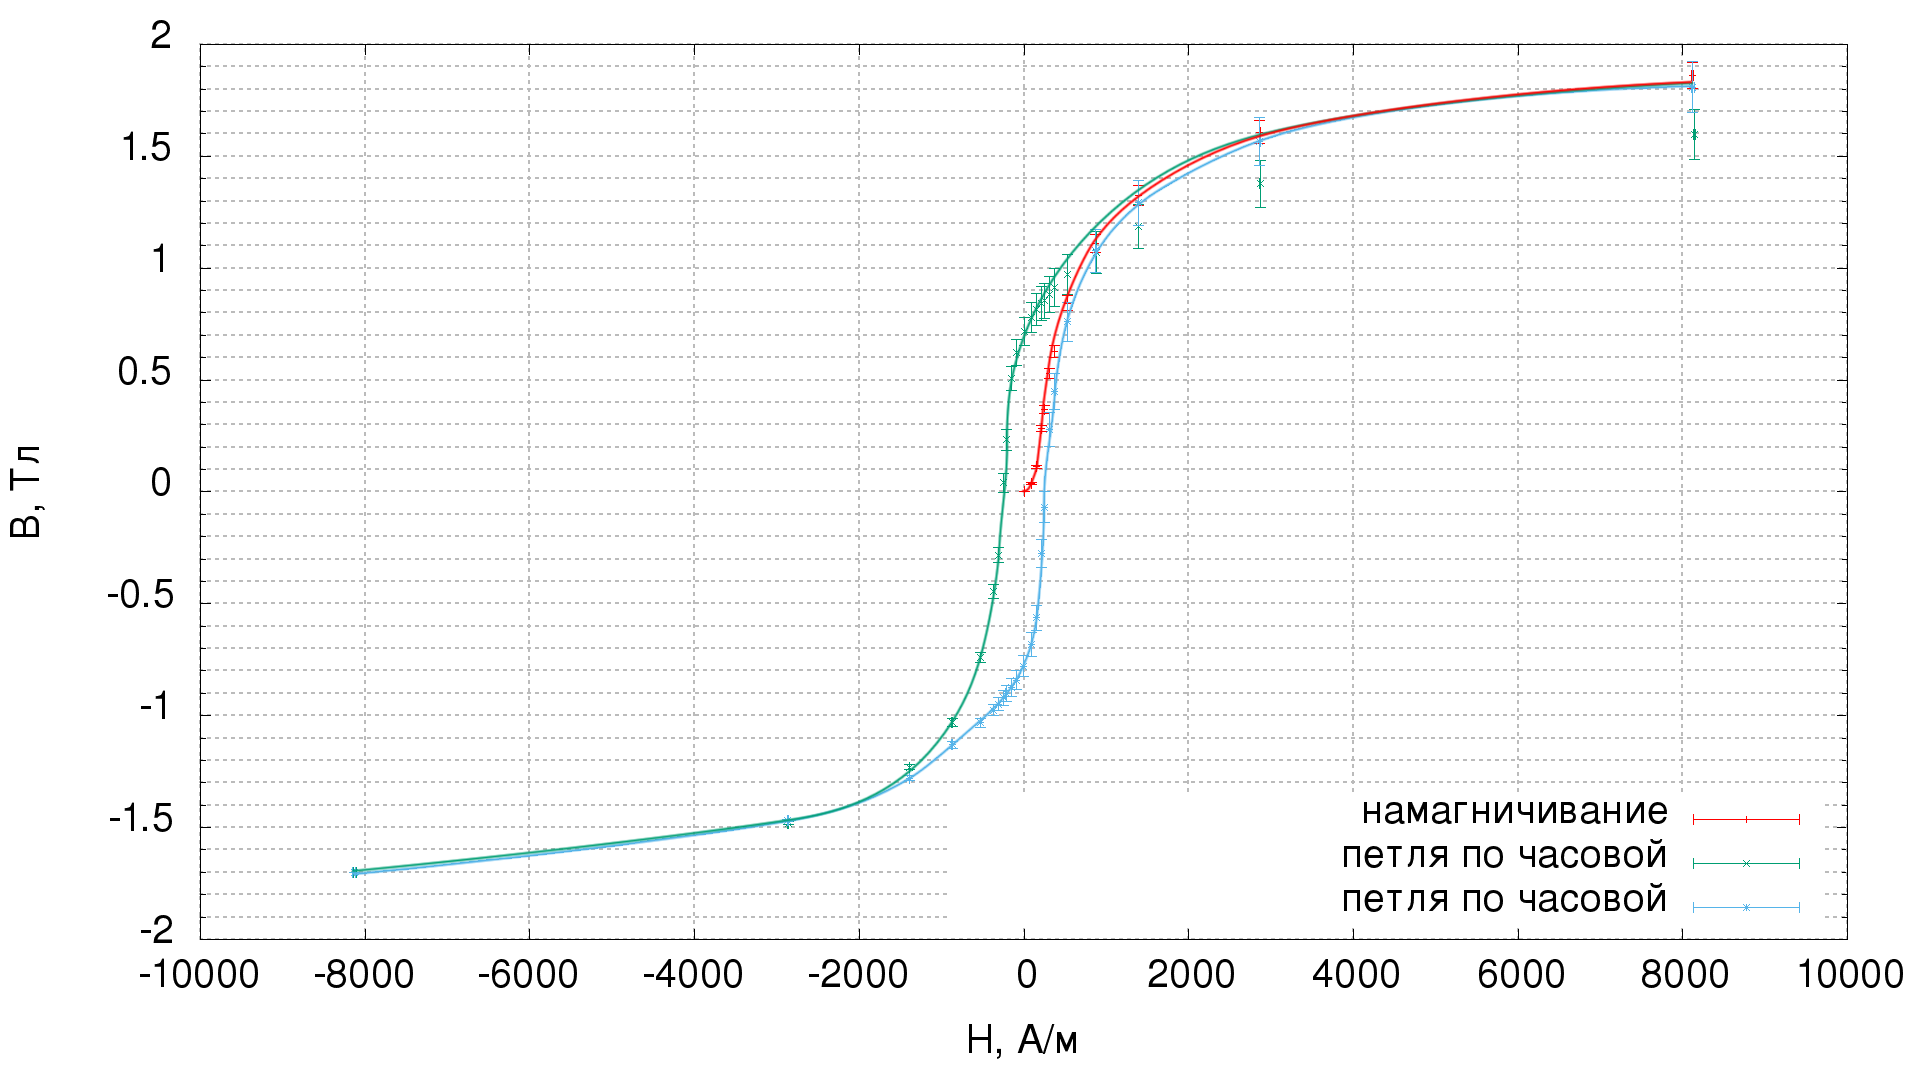
\includegraphics[width=0.99\textwidth]{5_big.png}
\end{center}
\begin{center}
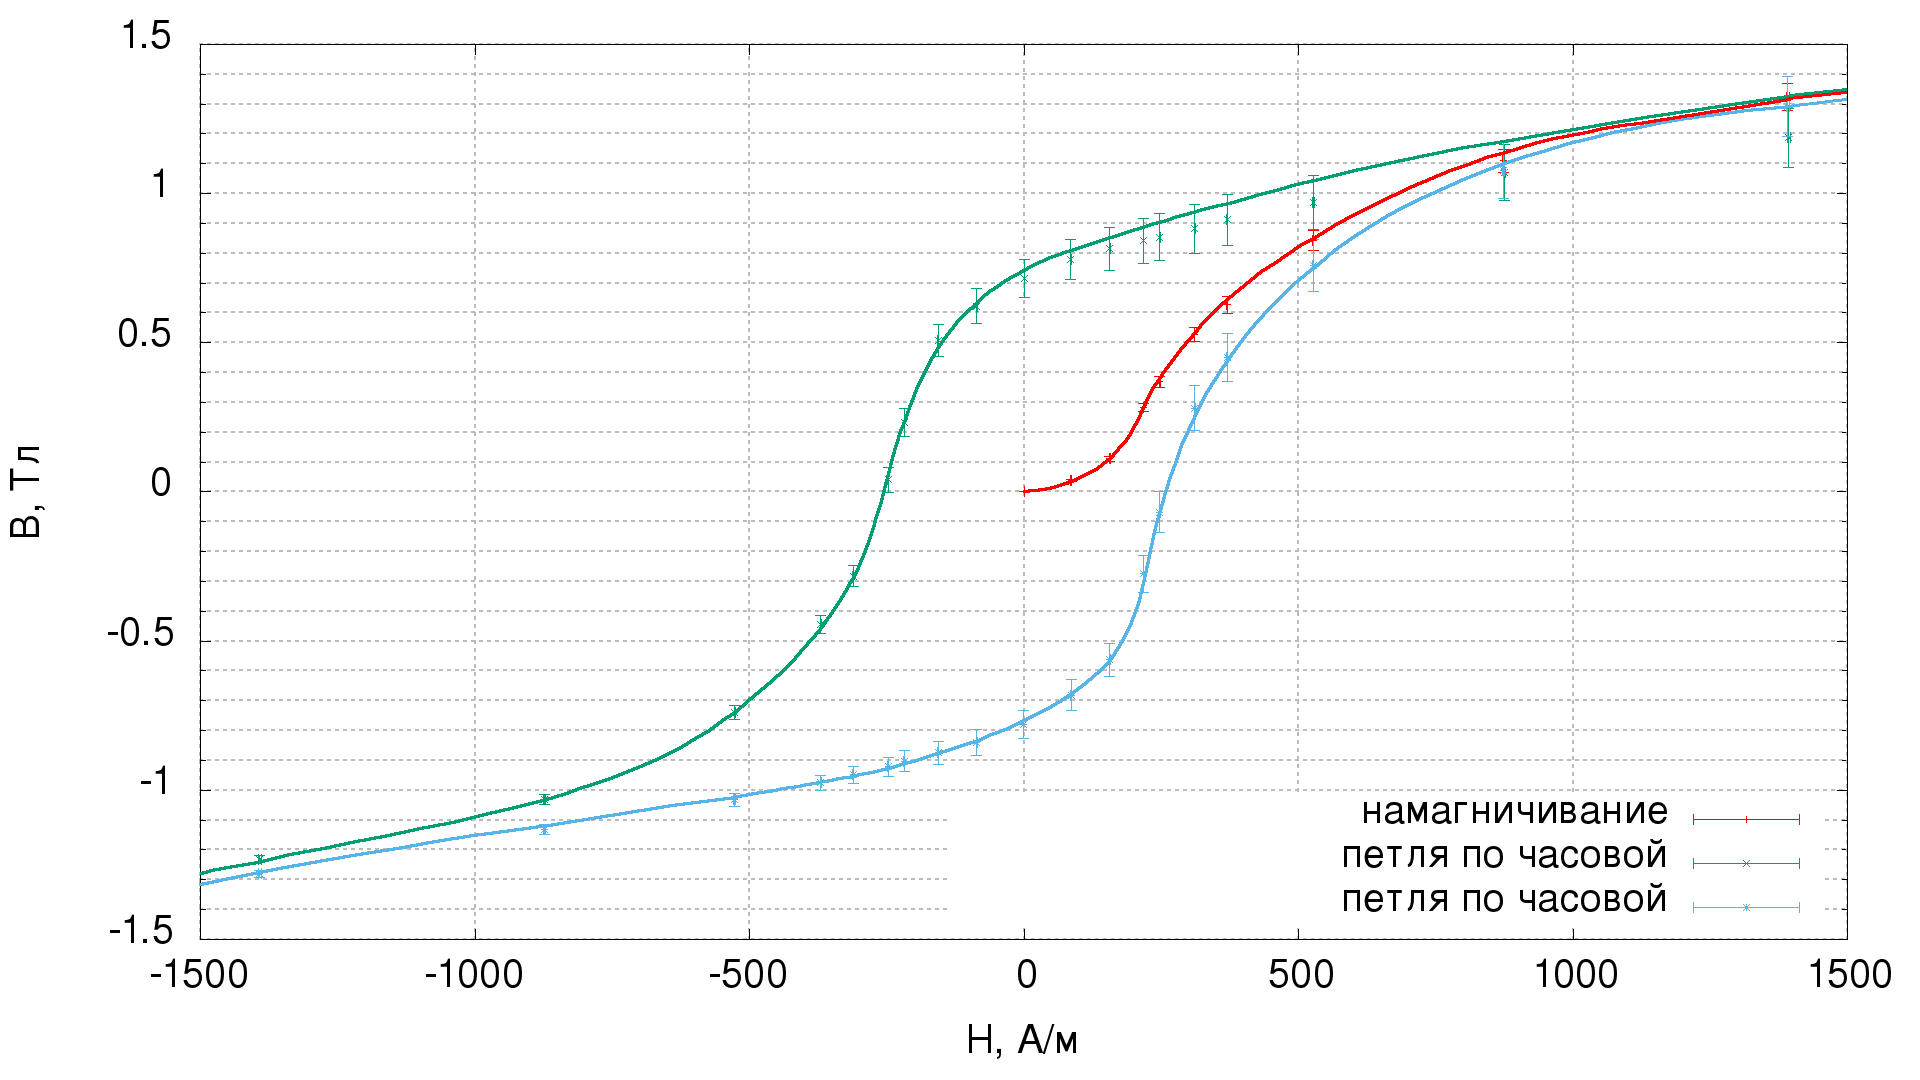
\includegraphics[width=0.99\textwidth]{5_small.png}
\end{center}

\subsection{обработка-4-6}

Из графиков:\\
Коэрцитивная сила $H_{c}=500*\frac{143\pm2}{275\pm2}\,\text{А}/\text{м} = 260\pm6\,\text{А}/\text{м}.$ (погрешность из толщины линии)\\
Индукция насыщения $B_s = (1.70\pm0.16)\,\text{Тл}$ (погрешность как корень суммы квадратов погрешности $\Delta B$ ($0.11\,\text{Тл}$) и половины разности между $B_s$ для разных направлений ($0.11\,\text{Тл}$)).

Для того, чтобы посчитать $\mu_\text{диф}$ я распечатал график, провел касательную и отсканировал график. Используя пропорции по пикселям я нашел :
$$\frac{dB}{dH} = \frac{1391-403\pm8}{2323-1856\pm8}\frac{3256-458\pm8}{1868-357\pm8}\frac{3\,\text{Тл}}{3000\,\text{А}/\text{м}} = (3.91\pm0.13) \frac{\text{мм}\,\text{Тл}}{\text{А}}.$$
$$\mu_\text{диф} = \frac{dB}{\mu_0dH} = 3100\pm100$$
График для демонстрации того, что я сделал, его почти полная копия выше.
\begin{center}
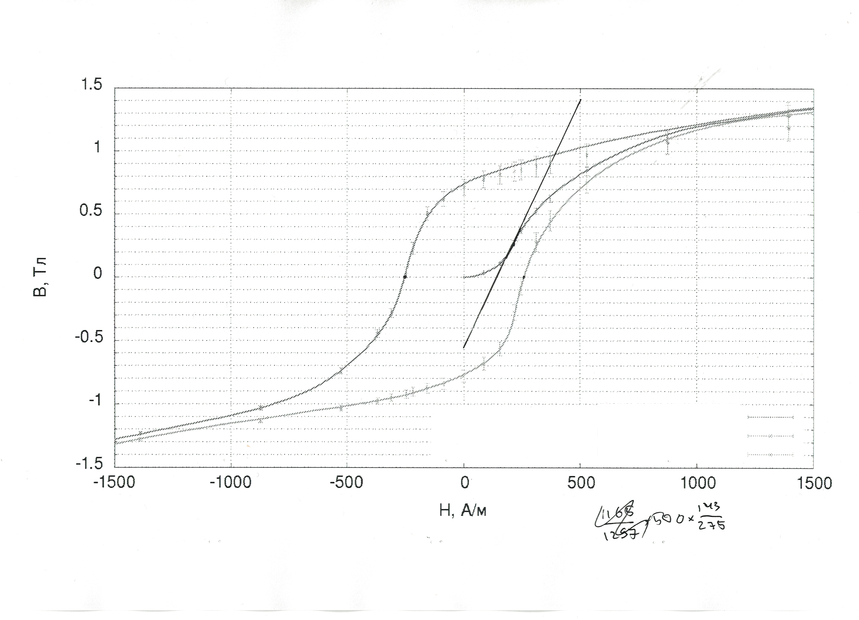
\includegraphics[width=0.99\textwidth]{6_res.png}
\end{center}

\begin{center}
\begin{tabular}{|c|c|c|}
\hline
&Эксперимент&таблица\\\hline
$\mu_\text{диф}$&$3100\pm100$&$5000$\\\hline
$B_s,\,\text{Тл}$&$1.70\pm0.16$&$2.15$\\\hline
$H_{c}\,\text{А}/\text{м}$&$260\pm6$&$80$\\\hline
\end{tabular}
\end{center}
\section*{Вывод}
Мы промерили петлю и кривую намагничивания у магнитного гистерезиса с помощью статического метода и получили значения индукции насыщения и дифференциальной магнитной проницаемости с отклонением от табличного значения менее чем на $30\%$ и $60\%$ соответственно, а также выяснили коэрцитивную силу менее, чем в $4$ раза превышающей табличное значение. Полученные отклонения я могу объяснить уникальностью характеристик установки, из-за чего реальные параметры могут сильно отличаться от табличных. 
\end{document}


125





\lipsum[1-4]
\begin{wrapfigure}{R}{5cm}
\centering
\includegraphics[width=0.20\textwidth]{rd.png}
\caption{1}
\end{wrapfigure}
\lipsum[1-6]


\begin{figure}[h]
\begin{center}$
\begin{array}{cccc}
\includegraphics[width=0.20\textwidth]{rd.png}&
\includegraphics[width=0.20\textwidth]{rd.png}&
\includegraphics[width=0.20\textwidth]{rd.png}&
\includegraphics[width=0.20\textwidth]{rd.png}\\
(1) & (2) & (3) & (4)
\end{array}$
\end{center}
\end{figure}
